Eine weitere Möglichkeit der Darstellung bietet die in der Aero-Toolbox implementierte Schnittstelle zwischen dem Flugsimulator FlightGear und \MatSim \cite{FGBlockDoku}. Bei FlightGear handelt es sich um eine Open-Source Software welche unter anderem zu Forschungszwecken und Pilotentraining entwickelt wurde. Die Schnittstelle von \MatSim zu FlightGear bietet damit die Möglichkeit einer möglichst realistischen Visualisierung von Flugbewegungen.
In \ref{fig:VisualFGBlock} sind die dafür nötigen Simulink-Blöcke gezeigt. Der erst Block benötigt die Eulerwinkel, Längen- und Breitengrad sowie die Flughöhe. Es können aber auch wie in \ref{label} beschreiben weitere Informationen wie zum Beispiel zu Geschwindigkeiten oder Antrieb und Treibstoff hinzugefügt werden.
Diese Informationen werden dann als so genanntes net-fdm-packet ausgegeben um anschließend mit dem zweiten Block an FlightGear gesendet zu werden. Dafür definiert man in den Blockparametern ein entsprechende Port sowie eine IP Adresse (vgl. \ref{fig:VisualFGBlockParam}).
Es gibt auch einen vorkonfigurierten Block, welcher die beiden beschriebenen Blöcke enthält. Da dieser jedoch zusätzlich einen Set-Pace-Block beinhaltet kann er nicht mehrfach in einem \MatSim Modell genutzt werden. Somit ist er nicht für Anwendungen geeignet bei denen mehrere Flugzeuge dargestellt werden sollen.
\begin{figure}[h]
	\centering
	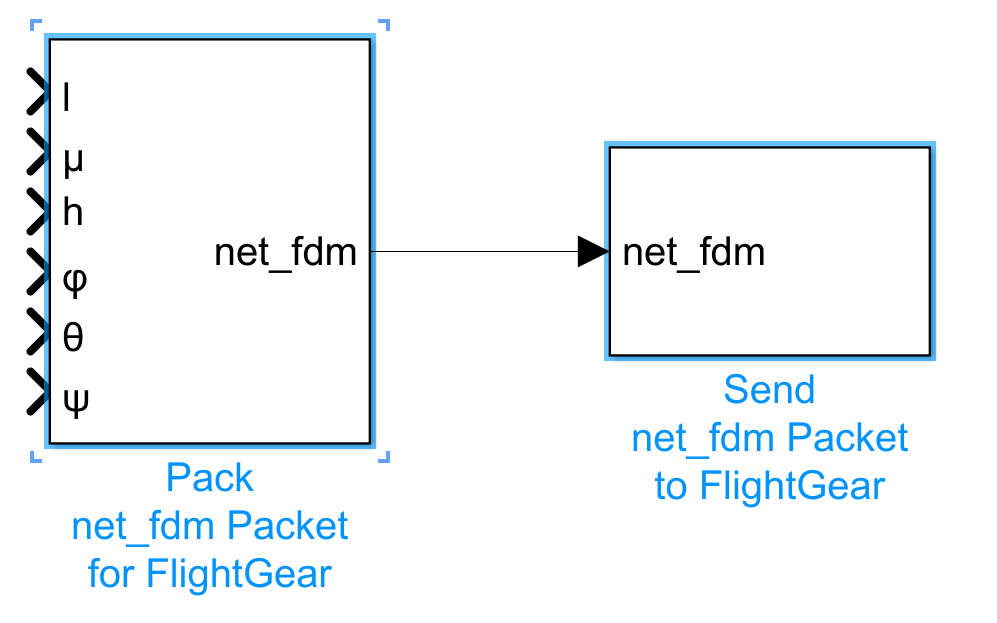
\includegraphics[width=\textwidth]{./Bilder/Visual_FGBlock.png}
	\caption{Simulink-Blöcke für Schnittstelle zu Flugsimulator FlightGear}
	\label{fig:VisualFGBlock}
\end{figure}
\begin{figure}[h]
	\centering
	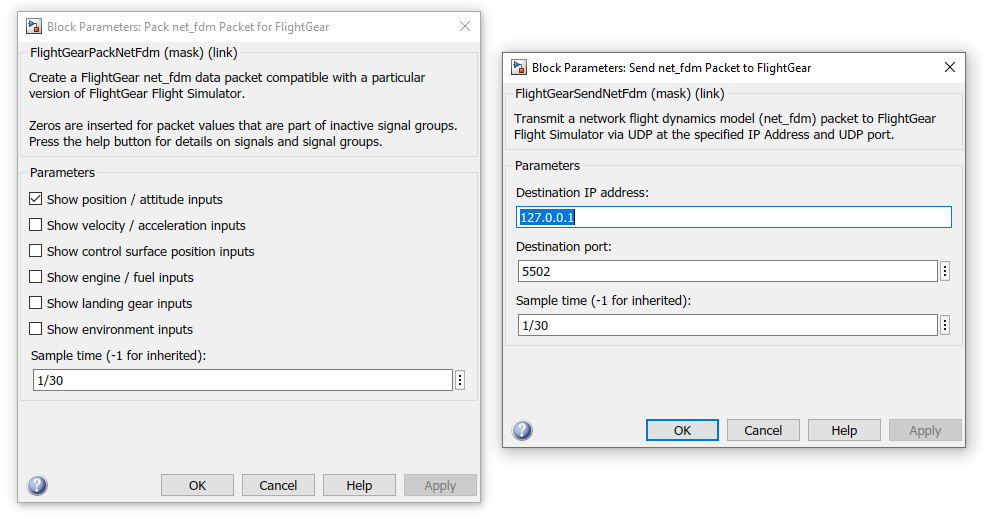
\includegraphics[width=\textwidth]{./Bilder/Visual_NetFdmBlockParam.png}
	\caption{Blockparameter für Simulink/FlightGear-Schnittstelle}
	\label{fig:VisualFGBlockParam}
\end{figure}

In FlightGear müssen dann die äquivalenten Einstellungen getroffen werden. Hierfür gibt es eine Kommandozeile in welche die Befehle in Codeform formuliert werden können. 
Möchte man mehrere Flugzeuge simulieren so kann man den Multiplayer-Modus nutzen um mehrere FlightGear-Instanzen zu verknüpfen. Dies geschieht entweder lokal oder auf einem offiziellen Server von FlightGear. Eine detailliertere Ausführung zu den möglichen Multiplayer-Einstellungen ist in \cite{How2Multi} zu finden.
Nachfolgender Code beschreibt beispielhaft die nötigen Eingaben in die FlightGear-Komandozeile.\\

Plane 1: --fdm=null --native-fdm=socket,in,30,localhost,5502,udp --multiplay=out,10,127.0.0.1,5000 --multiplay=in,10,127.0.0.1,5001 --callsign=Test1 \\

Plane 2: --fdm=null --native-fdm=socket,in,30,localhost,5503,udp --multiplay=out,10,127.0.0.1,5001 --multiplay=in,10,127.0.0.1,5000 --callsign=Test2\\


Plane 1: --fdm=null --native-fdm=socket,in,30,localhost,5502,udp --native-ctrls=socket,out,30,localhost,5505,udp --multiplay=out,10,mpserver01.flightgear.org,5000 --multiplay=in,30,,5000 --callsign=Test1 \\

Plane 2: --fdm=null --native-fdm=socket,in,30,localhost,5503,udp --native-ctrls=socket,out,30,localhost,5505,udp --multiplay=out,10,mpserver01.flightgear.org,5000 --multiplay=in,30,,5001 --callsign=Test2 \\

In Abbildung \ref{fig:VisualFG2Planes} ist ein Frame aus der FlightGear Animation gezeigt, welcher mit dieser Methode konzipiert wurde.
\begin{figure}[h]
	\centering
	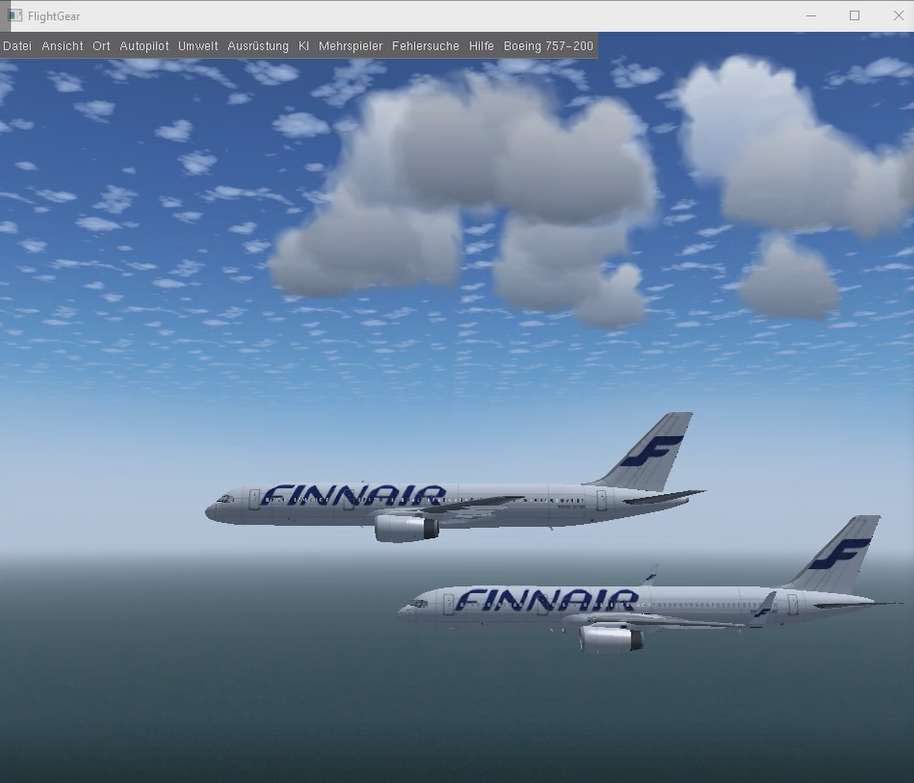
\includegraphics[width=\textwidth]{./Bilder/Visual_FG2Planes.png}
	\caption{Beispielanimation mit FlightGear}
	\label{fig:VisualFG2Planes}
\end{figure}
Aus einer breiten Bibliothek an Flugzeugen kann das für die Simulation benötigte ausgewählt werden. Zudem ist des möglich den Blickwinkel während der Animation anzupassen. Des weiteren ist durch den Horizont und die Wolken die Flugbahn der Flugzeuge besser nachvollziehbar. 

Jedoch tritt ein gravierendes Problem auf. Die Darstellung ruckelt und ist zeitlich verschoben. Damit ist sie für diese Arbeit ungenügend. Denn die Performance der Regelung kann nicht veranschaulicht werden, wenn die Flugzeuge in der Animation mehrere Meter hin und her springen. Die Ursache hierfür ist eine Asynchronität von \MatSim und den verschiedenen FlightGear-Instanzen.
Im Rahmen dieser Arbeit konnte dieses Problem nicht gelöst werden. In \cite{FGForum} wird ein mögliche Methode beschreiben um das Problem zu umgehen.
Dabei wird eine für diesen Zweck angepasste Version von FlightGear genutzt um die gesendeten Pakete auszulesen und mit einem Zeitstempel zu versehen. Somit kann eine flüssigere Animation erzielt werden.


%-> FG Blöcke + Impl Bsp:\\
%https://nl.mathworks.com/help/aeroblks/working-with-the-flight-simulator-interface.html
%
%Auch möglihc mehrer Flugzeuge dafür MultiPlayer\\
%Sub von FG Block da set Pace\\
%
%
%=> Problem keine saubere darstellung: Lag plus jitter\\
% Ursache: asynchronität von Packagerate Sim vs FG \\
% versuchte Lösungsansätze:\\
%  -rechenpower\\
%  -aufnahmen\\
%  -nicht lokal sondern Offi server\\
%  -Lag und Synch einstellungen\\
%  -red. der output rate / frame rate\\
%  
%  Nichts desto Trotz konnte im rahmen dieser Arbeit keine Lösung erarbeitet werden.\\
%
%
%Bilder:\\
%-Block in Matlab \\
%	.einfach\\
%    .für 2 Flugzeuge -> Set Pace Block\\
%- Einstellungsmenü in FG\\
%- flug in FG\\

 	
%REF:\\
%-Forum Markus: https://forum.flightgear.org/viewtopic.php?f=27&t=38421 	LABEL: FGForum\\
%-HowToMulti: https://wiki.flightgear.org/Howto:Multiplayer					LABEL: How2Multi\\
